\section{Auswertung}
\label{sec:Auswertung}

\subsection{Zeitabhängigkeit der Amplitude}

Die gemessenen Maxima bei einer gedämpften Schwingung sind 
in Tabelle \ref{tab:Messdaten1} zu sehen. 

\begin{table}
\centering
\caption{Messdaten der Maxima der Amplitude}
\label{tab:Messdaten1}
\sisetup{table-format=2.1}
\begin{tabular}{c c}
\toprule
$U \,/\, \si{\volt}$ & $s \,/\, \si{\micro\second}$\\
\midrule
1,74 &   0,0\\
1,44 &  29,6\\
1,20 &  58,8\\
1,10 &  88,2\\
0,84 & 117,2\\
0,68 & 147,2\\
0,56 & 177,2\\
0,46 & 206,2\\
0,38 & 235,2\\
0,30 & 265,2\\
0,22 & 294,2\\ 
0,16 & 324,2\\
0,14 & 353,2\\
0,10 & 382,2\\
0,06 & 412,2\\
0,02 & 441,2\\
0,00 & 471,2\\
\bottomrule
\end{tabular}
\end{table} 

Die Ausgleichsrechnung wird mit der Funktion 

\begin{equation*}
A = A_0 \cdot e^{-2\pi\mu t}
\end{equation*}

durchgeführt. Das Ergebnis ist in Abbildung \ref{fig:gedämpft} zu sehen. 

\begin{figure}
  \centering
  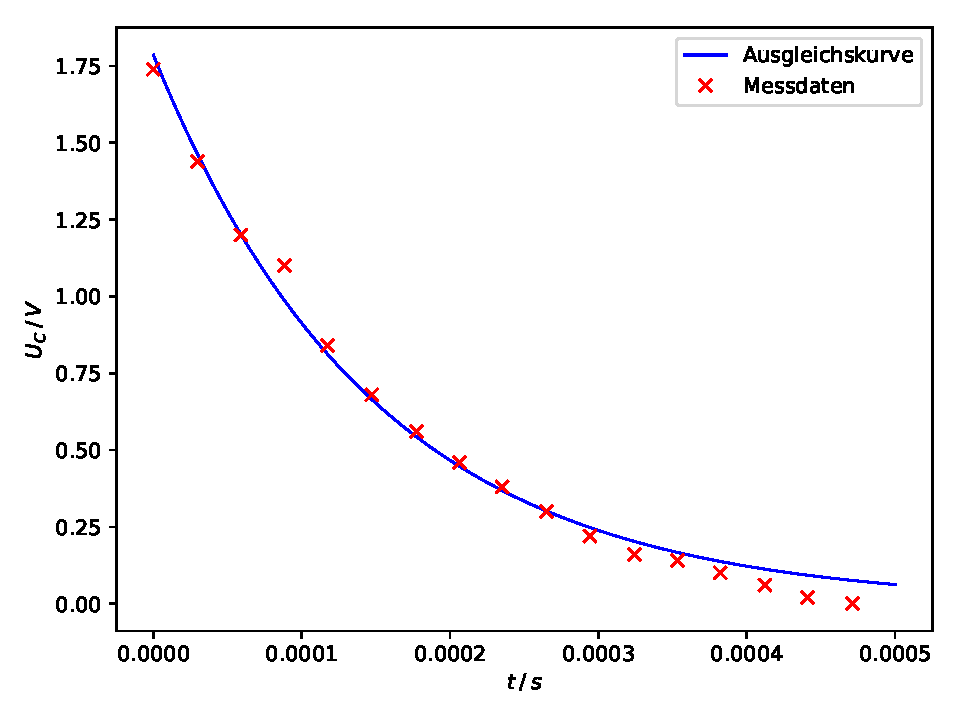
\includegraphics[scale=0.8]{content/plot1.pdf}
  \caption{Exponentielle Regression der Amplitude}
  \label{fig:gedämpft}
\end{figure}

Mittels python ergeben sich die Regressionsparamter zu: 

\begin{align*}
A_0 &= \SI{1.785+-0.036}{\volt},\\
\mu &= \SI{1068.421+-34.320}{\per\second}.
\end{align*}

Mit Formel... lässt sich nun der effiktive Widerstand berechnen.

\begin{equation*}
R_\text{eff} = 4\pi L\mu = \SI{136+-4}{\ohm}
\end{equation*}

Der Fehler ergibt sich dabei durch die Gaußsche Fehlerfortpflanzung zu: 

\begin{equation*}
\symup{\Delta} R_\text{eff} = \sqrt{\left(\frac{\symup{d}R_\text{eff}}{\symup{d}L}\right)²\cdot (\symup{\Delta}L)² +
\left(\frac{\symup{d}R_\text{eff}}{\symup{d}\mu}\right)²\cdot (\symup{\Delta}\mu)²}.
\end{equation*}

Weiterhin wird die Abklingdauer mit Formel... berechnet und 
es ergibt sich:

\begin{equation*}
T_\text{ex} = \frac{1}{2\pi\mu} = \SI{0.149+-0.005e-3}{\second}.
\end{equation*}

Der Fehler ergibt sich hierbei zu: 

\begin{equation*}
\symup{\Delta} T_\text{ex} = \sqrt{\left(\frac{\symup{d}T_\text{ex}}{\symup{d}\mu}\right)²\cdot (\symup{\Delta}\mu)²}.
\end{equation*}

\subsection{Bestimmung des Dämpfungswiderstandes}

Hier wurde der aperiodische Grenzfall untersucht. Dabei wurde der
Dämpfungswiderstand zu 

\begin{equation*}
R_\text{ap} = \SI{3520+-50}{\ohm}
\end{equation*}

bestimmt.
Der theoretische Wert von $R_\text{ap}$ kann mit Formel \eqref{eqn:apth} bestimmt 
werden: 

\begin{equation*}
R_\text{ap,theo} = \SI{4390+-9}{\ohm}.
\end{equation*}

Der Fehler berechnet sich über die Gaußsche Fehlerfortpflanzung: 

\begin{equation*}
\symup{\Delta} R_\text{ap,theo} = \sqrt{\left(\frac{\symup{d}R_\text{ap}}{\symup{d}L}\right)²\cdot (\symup{\Delta}L)² +
\left(\frac{\symup{d}R_\text{ap}}{\symup{d}C}\right)²\cdot (\symup{\Delta}C)²}.
\end{equation*}

\subsection{Frequenzabhängigkeit der Kondensatorspannung}

\begin{table}
  \centering
  \caption{Messdaten frequenzabhängigen Kondensatorspannung}
  \label{tab:Messdaten2}
  \sisetup{table-format=2.1}
  \begin{tabular}{c c c c}
  \toprule
  $f \,/\, \si{\kilo\hertz}$ & $U_C \,/\, \si{\volt}$ & $U \,/\, \si{\volt}$ & $\frac{U_C}{U} $\\
  \midrule
  09 & 1,08 & 0,56\\
  11 & 1,12 & 0,56\\
  13 & 1,16 & 0,56\\
  15 & 1,22 & 0,54\\
  17 & 1,30 & 0,56\\
  19 & 1,40 & 0,54\\
  21 & 1,56 & 0,56\\
  23 & 1,72 & 0,56\\
  25 & 1,96 & 0,56\\
  27 & 2,36 & 1,04\\
  29 & 2,84 & 0,96\\
  30 & 3,08 & 1,00\\
  31 & 3,40 & 1,00\\
  32 & 3,64 & 1,00\\
  33 & 3,72 & 1,00\\
  34 & 3,76 & 1,00\\
  35 & 3,56 & 1,00\\
  36 & 3,24 & 1,00\\
  37 & 2,92 & 1,00\\
  38 & 2,60 & 1,00\\
  39 & 2,28 & 1,00\\
  41 & 1,80 & 1,00\\
  43 & 1,48 & 1,04\\
  45 & 1,20 & 1,04\\
  47 & 0,98 & 0,52\\
  49 & 0,84 & 0,52\\
  51 & 0,74 & 0,52\\
  53 & 0,64 & 0,52\\
  55 & 0,59 & 0,21\\
  57 & 0,54 & 0,21\\
  59 & 0,49 & 0,21\\
  \bottomrule
  \end{tabular}
  \end{table} 